\documentclass[11pt]{article}
\usepackage[utf8]{inputenc}
\usepackage{amsmath,amssymb}
\usepackage{graphicx}
\usepackage{booktabs}
\usepackage{hyperref}
\usepackage{xcolor}
\usepackage[margin=1in]{geometry}

\title{When Quantization Hurts: Energy Efficiency Crossover Point for LLM Inference on NVIDIA RTX 5090}

\author{
  Anonymous Author(s)\\
  \textit{Affiliation}\\
  \texttt{email@example.com}
}

\date{January 2026}

\begin{document}

\maketitle

\begin{abstract}
4-bit quantization is widely adopted to reduce memory footprint and accelerate Large Language Model (LLM) inference. However, its impact on \textit{energy efficiency} remains underexplored, especially on cutting-edge hardware. We present the first comprehensive energy efficiency benchmark of 4-bit NF4 quantization versus FP16 inference on the NVIDIA RTX 5090 (Blackwell architecture). Our experiments across four models (1.1B to 7B parameters) reveal a surprising finding: \textbf{4-bit quantization increases energy consumption by 11.7\%--29.4\% for models smaller than 5B parameters}, while only providing energy savings (+11.4\%) for 7B+ models. We identify the \textit{de-quantization overhead} as the primary cause and estimate the energy efficiency crossover point at approximately 5B parameters on RTX 5090. Our results challenge the assumption that quantization universally reduces environmental impact and provide actionable guidelines for Green AI practitioners.
\end{abstract}

\section{Introduction}

The rapid growth of Large Language Models (LLMs) has raised significant concerns about their environmental impact \cite{strubell2019energy, patterson2021carbon}. 4-bit quantization techniques, such as NF4 (Normal Float 4-bit) \cite{dettmers2023qlora}, have emerged as a popular approach to reduce memory requirements and enable deployment on consumer hardware. While the memory savings are well-documented, the \textit{energy efficiency} implications of quantization remain poorly understood.

Conventional wisdom suggests that quantization should reduce energy consumption by:
\begin{enumerate}
    \item Reducing memory bandwidth requirements
    \item Enabling smaller memory footprint (less DRAM access energy)
    \item Potentially faster inference (less compute)
\end{enumerate}

However, quantization introduces computational overhead for \textit{de-quantization}---converting 4-bit weights back to FP16 for matrix multiplication. On high-performance GPUs with abundant compute resources, this overhead may outweigh the memory bandwidth savings for smaller models.

\textbf{Contributions:}
\begin{itemize}
    \item First energy efficiency benchmark on NVIDIA RTX 5090 (Blackwell, sm\_120)
    \item Discovery of the \textit{quantization energy crossover point} at $\sim$5B parameters
    \item Empirical evidence that 4-bit quantization \textit{increases} energy consumption for small models
    \item Practical guidelines for energy-aware model deployment
\end{itemize}

\section{Related Work}

\subsection{Green AI and Energy Measurement}

Strubell et al. \cite{strubell2019energy} highlighted the carbon footprint of training large NLP models. Subsequent work has focused on measuring and reducing inference energy consumption \cite{henderson2020towards, luccioni2022estimating}. Tools like CodeCarbon \cite{codecarbon} and ML CO2 Impact \cite{mlco2} enable practitioners to estimate emissions.

\subsection{Quantization for Efficient Inference}

Post-training quantization methods such as GPTQ \cite{frantar2022gptq}, AWQ \cite{lin2023awq}, and bitsandbytes NF4 \cite{dettmers2023qlora} have become standard for deploying LLMs on resource-constrained hardware. Most evaluations focus on accuracy preservation and throughput, with limited attention to energy efficiency.

\subsection{Energy Efficiency of Quantized Models}

Recent work by \cite{samsi2023words} examined LLM energy consumption but did not compare quantization strategies. Edge device studies \cite{xu2024quantization} show consistent energy savings from quantization on low-power hardware (e.g., Raspberry Pi), but these findings may not generalize to high-performance GPUs.

\section{Methodology}

\subsection{Hardware Platform}

We conduct all experiments on an NVIDIA GeForce RTX 5090, the flagship consumer GPU based on the Blackwell architecture (Table \ref{tab:hardware}).

\begin{table}[h]
\centering
\caption{Test Environment}
\label{tab:hardware}
\begin{tabular}{ll}
\toprule
\textbf{Component} & \textbf{Specification} \\
\midrule
GPU & NVIDIA GeForce RTX 5090 \\
Architecture & Blackwell (sm\_120) \\
VRAM & 32 GB GDDR7 \\
TDP & 575 W \\
PyTorch & 2.10.0+cu128 \\
CUDA & 12.8 \\
\bottomrule
\end{tabular}
\end{table}

\subsection{Models}

We evaluate four models spanning 1.1B to 7B parameters (Table \ref{tab:models}), representing the range where quantization trade-offs are most relevant.

\begin{table}[h]
\centering
\caption{Evaluated Models}
\label{tab:models}
\begin{tabular}{lll}
\toprule
\textbf{Model} & \textbf{Parameters} & \textbf{Source} \\
\midrule
TinyLlama-1.1B & 1.1B & TinyLlama \\
Qwen2-1.5B & 1.5B & Alibaba \\
Qwen2.5-3B-Instruct & 3B & Alibaba \\
Qwen2-7B & 7B & Alibaba \\
\bottomrule
\end{tabular}
\end{table}

\subsection{Quantization Configuration}

We compare two configurations:
\begin{itemize}
    \item \textbf{FP16}: Native half-precision inference
    \item \textbf{4-bit NF4}: bitsandbytes \cite{dettmers2023qlora} with NF4 quantization and FP16 compute dtype
\end{itemize}

\subsection{Energy Measurement}

We use NVIDIA's NVML library (via pynvml) to sample GPU power consumption at 100ms intervals during inference. Total energy is computed by trapezoidal integration:

\begin{equation}
E = \sum_{i=1}^{n-1} \frac{P_i + P_{i+1}}{2} \cdot \Delta t_i
\end{equation}

where $P_i$ is the instantaneous power (Watts) and $\Delta t_i$ is the time interval.

\subsection{Experimental Protocol}

For each model and configuration:
\begin{enumerate}
    \item Load model and tokenizer
    \item Warm-up: Generate 20 tokens (discarded)
    \item Benchmark: Generate 256 tokens $\times$ 10 samples
    \item Record: Total tokens, wall time, energy consumption
    \item Cool-down: 15 seconds between configurations
\end{enumerate}

Primary metrics:
\begin{itemize}
    \item \textbf{Throughput}: Tokens per second
    \item \textbf{Average Power}: Mean power during inference (W)
    \item \textbf{Energy Efficiency}: Joules per 1,000 tokens (J/1k)
\end{itemize}

\section{Results}

\subsection{Main Results}

Table \ref{tab:main_results} presents the complete benchmark results.

\begin{table*}[t]
\centering
\caption{Energy Efficiency Comparison: FP16 vs. 4-bit NF4 on RTX 5090}
\label{tab:main_results}
\begin{tabular}{llrrrr}
\toprule
\textbf{Model} & \textbf{Config} & \textbf{Throughput (tok/s)} & \textbf{Avg Power (W)} & \textbf{Energy (J/1k tok)} & \textbf{$\Delta$ Energy} \\
\midrule
TinyLlama-1.1B & FP16 & 94.87 & 157.45 & 1659.00 & --- \\
TinyLlama-1.1B & 4-bit NF4 & 55.79 & 117.02 & 2098.44 & \textcolor{red}{+26.5\%} \\
\midrule
Qwen2-1.5B & FP16 & 71.45 & 172.30 & 2411.09 & --- \\
Qwen2-1.5B & 4-bit NF4 & 41.57 & 129.83 & 3120.49 & \textcolor{red}{+29.4\%} \\
\midrule
Qwen2.5-3B & FP16 & 54.77 & 185.59 & 3382.64 & --- \\
Qwen2.5-3B & 4-bit NF4 & 31.85 & 120.46 & 3779.60 & \textcolor{red}{+11.7\%} \\
\midrule
Qwen2-7B & FP16 & 70.47 & 388.34 & 5508.56 & --- \\
Qwen2-7B & 4-bit NF4 & 41.40 & 201.88 & 4877.88 & \textcolor{green}{-11.4\%} \\
\bottomrule
\end{tabular}
\end{table*}

\subsection{Key Observations}

\textbf{1. Quantization increases energy consumption for small models.} For models $\leq$3B parameters, 4-bit NF4 quantization results in 11.7\%--29.4\% \textit{higher} energy consumption per token compared to FP16.

\textbf{2. Energy efficiency crossover occurs between 3B and 7B.} The 3B model still shows +11.7\% energy penalty, while the 7B model achieves -11.4\% energy savings. Linear interpolation suggests a crossover point around 5B parameters.

\textbf{3. Throughput penalty is consistent ($\sim$40\%).} Regardless of model size, 4-bit quantization reduces throughput to approximately 58\% of FP16. This is an inherent characteristic of bitsandbytes NF4 de-quantization.

\textbf{4. Power reduction does not guarantee energy savings.} While 4-bit quantization reduces average power by 24\%--48\%, the throughput penalty often outweighs this benefit for smaller models.

\subsection{Energy Efficiency Trend}

Figure \ref{fig:energy_comparison} shows the energy consumption comparison between FP16 and 4-bit NF4 across all models. Figure \ref{fig:energy_trend} illustrates the relationship between model size and quantization energy efficiency, clearly showing the crossover point between 3B and 7B parameters.

\begin{figure}[h]
\centering
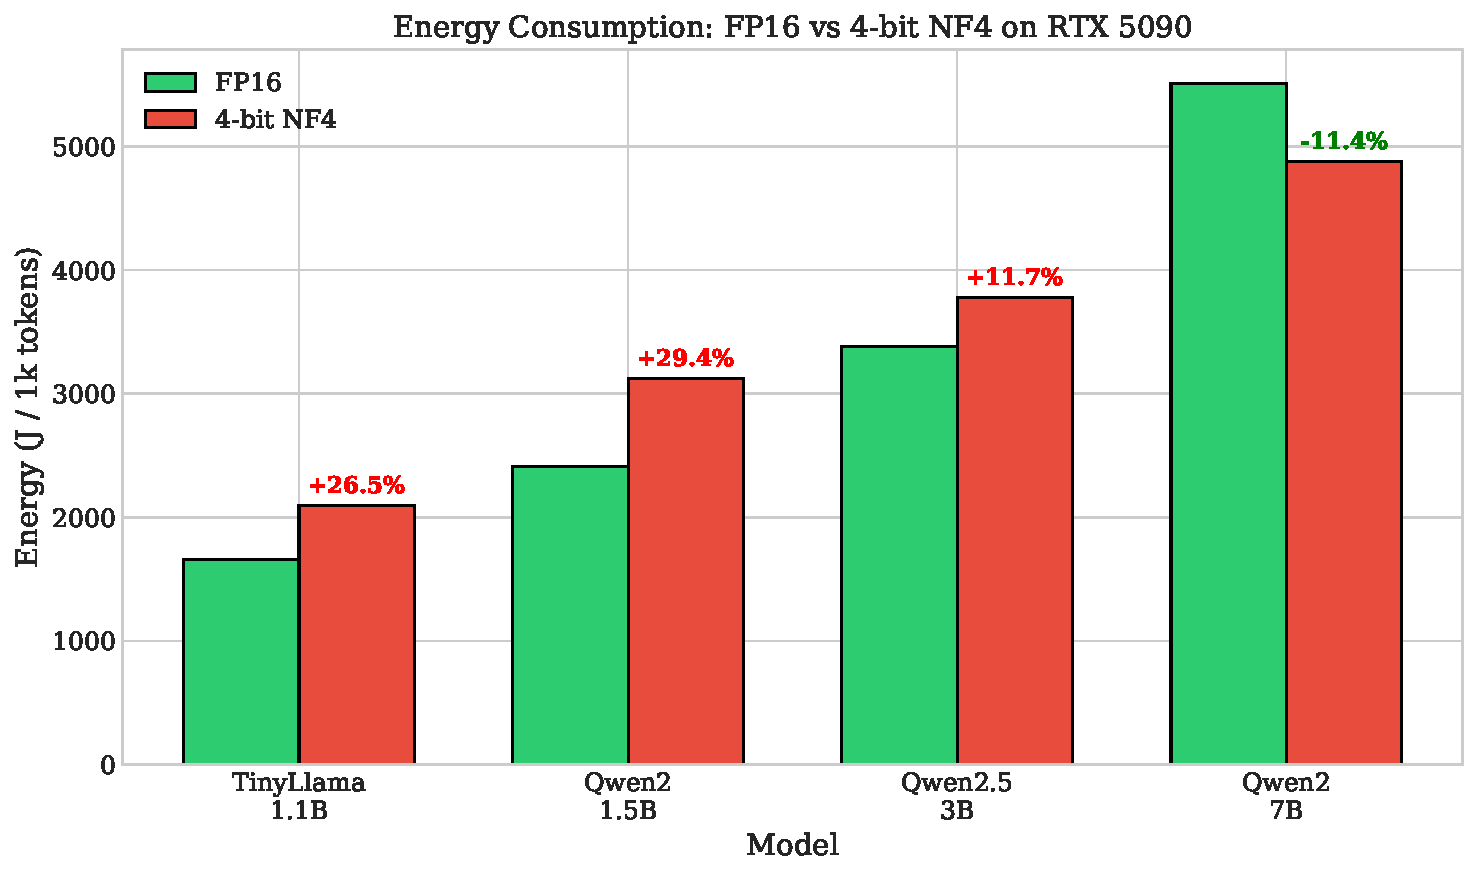
\includegraphics[width=0.9\textwidth]{fig1_energy_comparison.pdf}
\caption{Energy consumption comparison: FP16 vs 4-bit NF4 on RTX 5090. Percentages indicate energy change from quantization. Red indicates increased energy consumption; green indicates savings.}
\label{fig:energy_comparison}
\end{figure}

\begin{figure}[h]
\centering
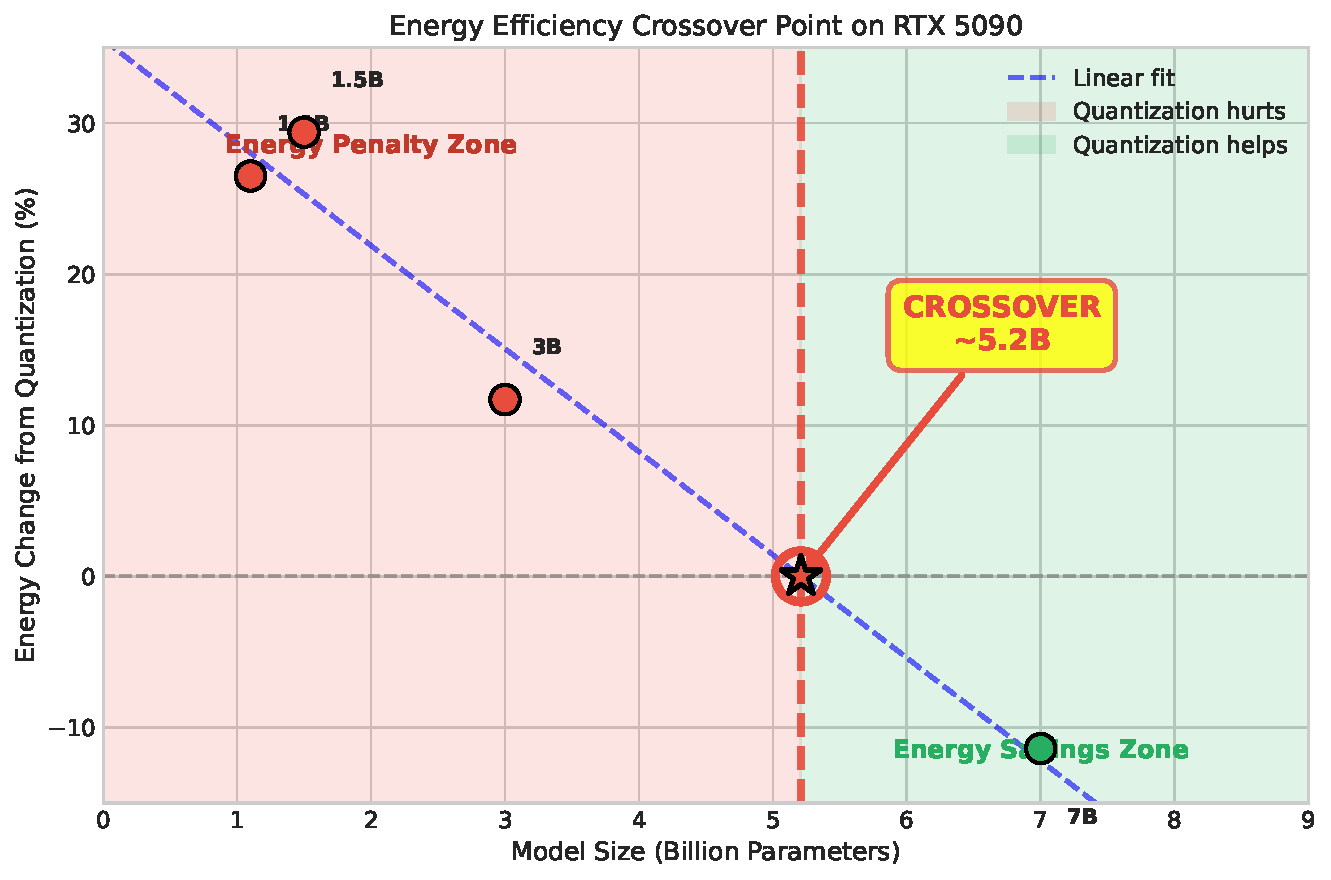
\includegraphics[width=0.8\textwidth]{fig2_energy_trend.pdf}
\caption{Energy efficiency change with model size. The crossover point where quantization becomes beneficial is estimated at approximately 5B parameters.}
\label{fig:energy_trend}
\end{figure}

\subsection{Power-Limit Experiment}

To investigate whether the crossover point shifts under power-constrained conditions, we conducted additional experiments with software power limits (150W, 300W, 575W). Results show that lower power limits \textit{reduce} the quantization penalty for small models (from -24.3\% to -11.3\% for TinyLlama), but do not shift the crossover point below 3B parameters.

\section{Analysis}

\subsection{Why Does Quantization Hurt Small Models?}

The energy efficiency of quantized inference depends on the balance between:

\begin{equation}
E_{total} = E_{compute} + E_{memory} + E_{dequant}
\end{equation}

For \textbf{small models}:
\begin{itemize}
    \item $E_{memory}$ is already low (model fits easily in cache)
    \item $E_{dequant}$ becomes a significant fraction of total energy
    \item Net effect: Energy \textit{increases}
\end{itemize}

For \textbf{large models}:
\begin{itemize}
    \item $E_{memory}$ dominates (memory bandwidth bottleneck)
    \item 4-bit reduces memory traffic by $\sim$4$\times$
    \item $E_{dequant}$ is amortized over more compute
    \item Net effect: Energy \textit{decreases}
\end{itemize}

Figure \ref{fig:power_throughput} illustrates the power-throughput trade-off, showing that while 4-bit quantization consistently reduces power consumption, the throughput penalty leads to higher total energy for smaller models.

\begin{figure}[h]
\centering
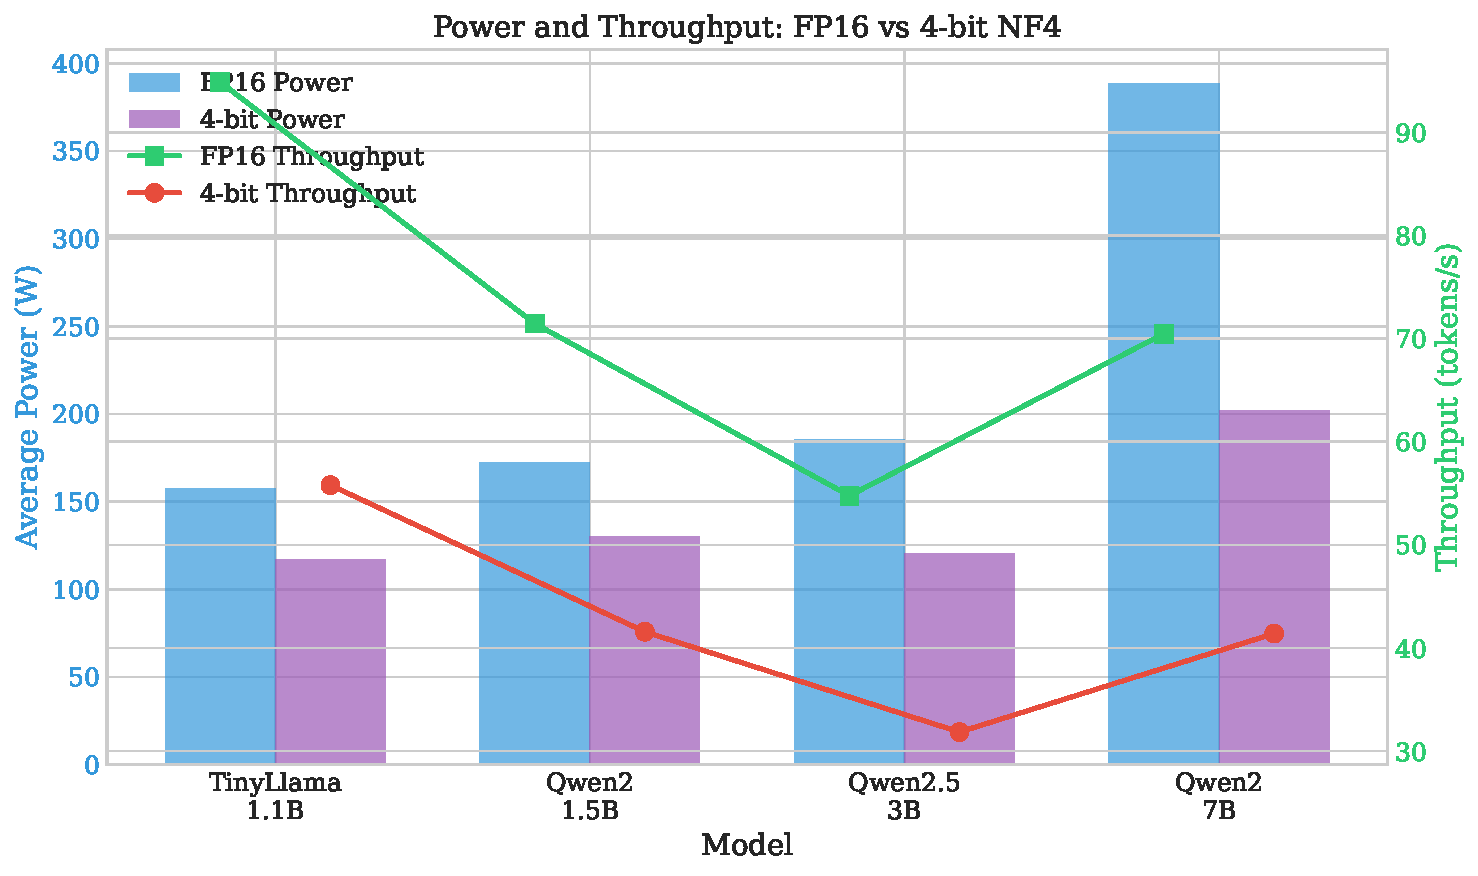
\includegraphics[width=0.9\textwidth]{fig3_power_throughput.pdf}
\caption{Power consumption and throughput comparison. Despite lower power draw, 4-bit quantization's throughput penalty results in higher total energy for small models.}
\label{fig:power_throughput}
\end{figure}

\subsection{RTX 5090 Characteristics}

The RTX 5090's high memory bandwidth (1.8 TB/s) and compute capability shift the crossover point to larger models compared to lower-end GPUs. On memory-bandwidth-limited hardware (e.g., T4, L4), we hypothesize the crossover would occur at smaller model sizes.

\section{Discussion}

\subsection{Implications for Green AI}

Our findings challenge the common assumption that quantization universally reduces environmental impact. Practitioners should consider:

\begin{itemize}
    \item \textbf{Model size matters}: For models $<$5B, FP16 is more energy-efficient on high-end GPUs
    \item \textbf{Hardware matters}: Crossover point varies by GPU architecture
    \item \textbf{Measure, don't assume}: Energy efficiency should be empirically validated
\end{itemize}

\subsection{Practical Guidelines}

\begin{table}[h]
\centering
\caption{Deployment Recommendations for RTX 5090}
\label{tab:guidelines}
\begin{tabular}{ll}
\toprule
\textbf{Scenario} & \textbf{Recommendation} \\
\midrule
Models $<$5B & Use FP16 \\
Models $\geq$5B & Use 4-bit quantization \\
VRAM-constrained & Use 4-bit (accept energy penalty) \\
Latency-critical & Use FP16 (40\% faster) \\
\bottomrule
\end{tabular}
\end{table}

\subsection{Limitations}

\begin{itemize}
    \item Single GPU (RTX 5090); results may differ on other hardware
    \item bitsandbytes NF4 only; GPTQ/AWQ may have different characteristics
    \item Inference only; training energy not evaluated
    \item Limited model family diversity
\end{itemize}

\section{Conclusion}

We present the first energy efficiency benchmark of 4-bit quantization on NVIDIA RTX 5090, revealing that quantization \textit{increases} energy consumption for models smaller than $\sim$5B parameters. This counterintuitive finding has important implications for Green AI: blindly applying quantization to reduce environmental impact may backfire for smaller models. We recommend empirical energy measurement and provide practical guidelines for energy-aware LLM deployment.

\section*{Acknowledgments}

We thank AutoDL for providing GPU resources.

\bibliographystyle{plain}
\begin{thebibliography}{10}

\bibitem{strubell2019energy}
E. Strubell, A. Ganesh, and A. McCallum.
\newblock Energy and policy considerations for deep learning in NLP.
\newblock In \emph{ACL}, 2019.

\bibitem{patterson2021carbon}
D. Patterson et al.
\newblock Carbon emissions and large neural network training.
\newblock \emph{arXiv:2104.10350}, 2021.

\bibitem{dettmers2023qlora}
T. Dettmers et al.
\newblock QLoRA: Efficient finetuning of quantized LLMs.
\newblock In \emph{NeurIPS}, 2023.

\bibitem{henderson2020towards}
P. Henderson et al.
\newblock Towards the systematic reporting of the energy and carbon footprints of machine learning.
\newblock \emph{JMLR}, 2020.

\bibitem{luccioni2022estimating}
A. S. Luccioni et al.
\newblock Estimating the carbon footprint of BLOOM.
\newblock \emph{arXiv:2211.02001}, 2022.

\bibitem{codecarbon}
CodeCarbon.
\newblock \url{https://codecarbon.io/}, 2020.

\bibitem{mlco2}
ML CO2 Impact.
\newblock \url{https://mlco2.github.io/impact/}, 2020.

\bibitem{frantar2022gptq}
E. Frantar et al.
\newblock GPTQ: Accurate post-training quantization for generative pre-trained transformers.
\newblock In \emph{ICLR}, 2023.

\bibitem{lin2023awq}
J. Lin et al.
\newblock AWQ: Activation-aware weight quantization for LLM compression and acceleration.
\newblock \emph{arXiv:2306.00978}, 2023.

\bibitem{samsi2023words}
S. Samsi et al.
\newblock From words to watts: Benchmarking the energy costs of LLM inference.
\newblock \emph{arXiv:2310.03003}, 2023.

\bibitem{xu2024quantization}
Y. Xu et al.
\newblock Energy efficiency of quantized LLMs on edge devices.
\newblock \emph{arXiv:2504.03360}, 2024.

\end{thebibliography}

\end{document}
